\documentclass[12pt,a4paper]{ctexart}

\usepackage[UTF8]{ctex}
\usepackage{geometry}
\usepackage{graphicx}
\usepackage{xcolor}
\usepackage{tikz}
\usepackage{fontspec}
\usepackage{setspace}
\usepackage{enumitem}
\usepackage{booktabs}
\usepackage{array}
\usepackage{longtable}
\usepackage{hyperref}
\usepackage{fancyhdr}
\usepackage{titlesec}
\usepackage{multicol}
\usepackage{xurl}
\usepackage{tocloft}

\renewcommand{\cfttoctitlefont}{\hfill\bfseries\Large}
\renewcommand{\cftaftertoctitle}{\hfill}
\geometry{left=2.5cm,right=2.5cm,top=2.5cm,bottom=2.5cm}

\definecolor{black}{RGB}{0,0,0}
\definecolor{mainblue}{RGB}{0,82,147}
\definecolor{accentgold}{RGB}{180,140,60}
\definecolor{lightgray}{RGB}{245,245,245}
\definecolor{darkgray}{RGB}{80,80,80}
\definecolor{mainred}{RGB}{230,1,45}

\hypersetup{
    colorlinks=true,
    linkcolor=black,
    urlcolor=mainblue,
    citecolor=mainblue,
    pdfborder={0 0 0}
}

\pagestyle{fancy}
\fancyhf{}
\fancyhead[L]{\small\color{darkgray}\textbf{量子行业每周新闻洞察}}
\fancyhead[R]{\small\color{darkgray}\textbf{总第191期}}
\fancyfoot[C]{\thepage}
\renewcommand{\headrulewidth}{0.4pt}
\renewcommand{\footrulewidth}{0pt}

\titleformat{\section}
    {\Large\bfseries\color{mainred}}
    {\thesection、}{0em}{}
\titleformat{\subsection}
    {\large\bfseries\color{mainred}}
    {\thesubsection、}{0em}{}

\newcolumntype{L}[1]{>{\raggedright\arraybackslash}p{#1}}
\newcolumntype{C}[1]{>{\centering\arraybackslash}p{#1}}

\begin{document}

% ==================== 封面 ====================
\begin{titlepage}
\begin{tikzpicture}[remember picture,overlay]
    \fill[mainred] ([yshift=-0.5cm]current page.north west) rectangle ([yshift=-1.2cm]current page.north east);
    \fill[mainred] ([yshift=1.2cm]current page.south west) rectangle ([yshift=0.5cm]current page.south east);
\end{tikzpicture}

\vspace*{4cm}

\begin{center}
    {\fontsize{44}{52}\selectfont\bfseries\color{black} \textbf{量子行业每周新闻洞察}}

    \vspace{0.8cm}

    {\fontsize{16}{22}\selectfont\color{darkgray} 2026.08.02 — 2026.08.07 }
    {\fontsize{16}{22}\selectfont\color{darkgray} \textbf{WEEKLY NEWS}}

    \vspace{1.5cm}

    {\fontsize{20}{26}\selectfont\color{mainred}\textbf{（总第\textbf{ 191 }期）}}

    \vspace{4cm}

    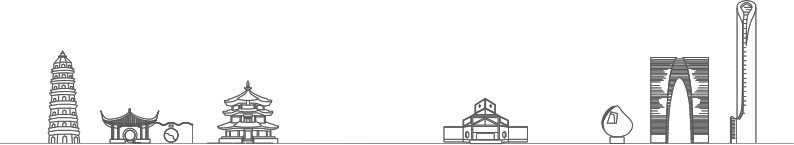
\includegraphics[width=\textwidth]{Cover_Suzhou.png}

    \vfill

    {\fontsize{12}{16}\selectfont\color{darkgray} 量子科技长三角产业创新中心\\编制：科技委办公室、产业发展部（理事会办公室）}
\end{center}
\end{titlepage}

% ==================== 目录 ====================
\pagenumbering{roman}
\newpage
\tableofcontents

\newpage

% ==================== 摘要 ====================
\pagenumbering{arabic}
\setcounter{page}{1}
\begin{center}
{\Large\bfseries\color{mainred} 摘\hspace{2em}要}
\end{center}
\addcontentsline{toc}{section}{摘要}


\textbf{ 宏观态势：}

量子技术正加速从实验室走向国家战略基础设施层面。各国竞相布局的核心逻辑趋同——政府主导、产业协同、生态先行。以色列启动国家量子计算平台招标，泰国以俱乐部模式推动区域量子经济，德国则更注重前沿探索与基础设施联动，QTF倡议中的全国光纤骨干网构想尤为值得关注，其本质是为量子通信与分布式计算铺设底层“高速公路”。国内工信部量子信息标准化技术委员会的成立，标志着中国在量子技术规范化、产业化进程中迈出关键一步，标准先行有利于抢占话语权。


\textbf{ 科技前沿：}

本周科研突破呈现“纠错、编码、物理实现”三线并进的格局，且成果密集登上《自然》等顶刊。微软与D-Wave在量子纠错和门保真度上取得里程碑式进展，直接推动容错量子计算走向实用化；加州理工与康奈尔在编码和光子操控上的创新，则为提升计算效率和扩展信息传输维度提供了全新工具。值得关注的是，国内团队在离子纠缠生成、室温单电子操控以及量子赋能AI医疗上的表现，显示中国在原始创新与交叉应用层面正同步发力，量子技术对现实产业的反哺效应开始显现。


\textbf{ 产品动态：}

行业正从“验证技术”转向“交付工具”，强调可用性与教育普及。QuiX Quantum将光子处理器商业化是迈向专用量子计算平台的关键一步；德国SAXON Q开放数百比特级量子计算机订购，标志供给端开始提供更大规模的服务能力。印度高校引入量子硬件用于教学，QNu Labs则着手培训师资，显示产业链已延伸至人才培养环节。此外，量子神经网络首次跨平台验证，表明算法在不同硬件间的可移植性取得突破，这为未来软硬解耦、生态互通奠定了重要基础。


\textbf{ 企业资讯：}

产业链整合与跨界协作大幅提速，量子技术正深度融入国家安全与工业应用场景。IonQ与桑迪亚实验室及NRO的双重合作，是量子技术切入国防与情报领域的重要信号；三菱电机投资量子优化公司、富士通联合澳洲机构搞研发，凸显传统工业巨头对量子赋能降本增效的迫切需求。国际方面，日澳签署合作备忘录，量子供应链正呈现区域化联盟趋势。国内则通过湖北研企联合平台等模式，探索科技成果转化的新路径，整体而言，量子技术的商用化、产业化和安全化导向愈发清晰。


\textbf{ 资本运作：}

成熟公司与初创企业在融资与商业模式上呈现冰火两重天的分化，但市场对量子赛道的长期信心未减。IonQ营收大增但净亏损持续，Xanadu营收微薄且亏损扩大，表明头部公司仍处于高投入换增长阶段。IQM在手订单破亿欧元，则印证了超导路线的商业化潜力正在兑现。初创端融资热度极高，幺正量子四个月内完成A轮、多个量子项目获数千万元级融资，资本正密集押注具备原创算法和核心硬件能力的团队，量子计算硬科技投资进入深水区。




\textbf{ 专利动态：}

本周专利动态涵盖量子软件与算法共1个板块、8条专利。




% ==================== 会议列表 ====================
{
    \newpage
    \section*{ 8月量子科技行业国内、国际会议}
    \addcontentsline{toc}{section}{ 8月量子科技行业国内、国际会议}
    \scriptsize
    \begin{longtable}{C{0.8cm}L{2.5cm}L{3cm}L{7cm}}
        \toprule[1.5pt]
        \textbf{序号} & \textbf{日期} & \textbf{地点} & \textbf{会议名称} \\
        \midrule
        \endfirsthead
        \toprule
        \textbf{序号} & \textbf{日期} & \textbf{地点} & \textbf{会议名称} \\
        \midrule
        \endhead
        \bottomrule
        \endfoot
        
        1 & 8月3日-5日 & 博尔德及线上, 美国 & 天气与气候应用的量子计算与传感研讨会 \\
        \midrule[0.05pt]
        
        2 & 8月3日-14日 & 贝纳斯克, 西班牙 & 容错量子技术研讨会 \\
        \midrule[0.05pt]
        
        3 & 8月7日-9日 & 杭州, 中国 & 第2届量子计算与通信技术国际会议（ICQCT 2026） \\
        \midrule[0.05pt]
        
        4 & 8月10日-14日 & 纳塔尔, 巴西 & 量子热力学会议2026（QTD 2026） \\
        \midrule[0.05pt]
        
        5 & 8月10日-14日 & 阿姆斯特丹, 荷兰 & QSim2026 \\
        \midrule[0.05pt]
        
        6 & 8月14日-16日 & 印第安纳波利斯, 美国 & 量子AI与自然语言处理2026会议（QNLPAI 2026） \\
        \midrule[0.05pt]
        
        7 & 8月16日-21日 & 巴德洪内夫, 德国 & 量子机器学习暑期学校（Bad Honnef物理学校） \\
        \midrule[0.05pt]
        
        8 & 8月16日-22日 & 贝纳斯克, 西班牙 & 悬浮系统量子工程研讨会 \\
        \midrule[0.05pt]
        
        9 & 8月17日-21日 & 多伦多, 加拿大 & 第11届量子信息与量子控制会议（CQIQC-XI） \\
        \midrule[0.05pt]
        
        10 & 8月17日-21日 & 阿姆斯特丹, 荷兰 & 第23届量子物理与逻辑国际会议（QPL 2026） \\
        \midrule[0.05pt]
        
        11 & 8月24日-28日 & 渥太华, 加拿大 & QCrypt 2026 \\
        \midrule[0.05pt]
        
        12 & 8月24日-28日 & 大田, 韩国 & 第26届亚洲量子信息科学会议 (AQIS) \\
        \midrule[0.05pt]
        
        13 & 8月24日-28日 & 维也纳, 奥地利 & 第9届青年量子信息科学家国际会议 (YQIS) \\
        \midrule[0.05pt]
        
        14 & 8月25日-28日 & 哥德堡, 瑞典 & 超导量子比特与算法 2026 (SQA) \\
        \midrule[0.05pt]
        
        15 & 8月30日-9月1日 & 布雷钦, 英国 & 量子ARC写作静修 \\
        \midrule[0.05pt]
        
        16 & 8月31日-9月3日 & 仁川, 韩国 & 硅量子电子学研讨会 2026 (SiQEW) \\
        \midrule[0.05pt]
        
        17 & 8月31日-9月3日 & 泰恩河畔纽卡斯尔, 英国 & Photon 2026 \\
        \midrule[0.05pt]
        
        18 & 8月31日-9月4日 & 瓦莱塔, 马耳他 & Qalypso 2026暑期学校—量子优化技术与计算物理 \\
        \midrule[0.05pt]
        
        19 & 8月31日-9月4日 & 舍布鲁克, 加拿大 & 量子计算、通信与密码学理论 2026 (TQC) \\
        \midrule[0.05pt]
        
        20 & 8月31日-9月10日 & 格但斯克, 波兰 & Q-Camp: 量子暑期学校 2026 \\
        \midrule[0.05pt]
        
    \end{longtable}
}




% ==================== 宏观态势 ====================
\newpage
\section{宏观态势}
\vspace{-0.5em}
\noindent\rule{\linewidth}{1.5pt}

\subsection{ 以色列启动国家量子计算平台招标 将打造本土量子计算系统 }

2026年08月07日消息，以色列总理办公室国家人工智能局与财政部总会计师司宣布，启动一项国家级招标，以建设本土量子计算平台“Project Nexus”。据悉，该平台将被打造成一台完全在以色列本土设计制造的名为“蓝白”的量子计算系统，旨在确保以色列拥有自产量子计算机，同时支持国内科研与产业生态生态中已开展的多条量子技术路线。此次招标还包含多项新的人工智能相关计划。此举被视为以色列强化技术主权、保持先进计算与人工智能领域竞争力的重要举措。

\noindent\textbf{报道链接：}\url{https://thequantuminsider.com/2026/08/05/israel-launches-national-quantum-computer-tender-as-part-of-broader-ai-sovereignty-strategy/}

\subsection{ 泰国多家机构联合qBraid成立泰国量子俱乐部 四大优先领域布局量子经济 }

2026年08月06日消息，泰国高等教育、科研与创新部（MHESI）联合正大集团等企业及美国量子软件平台商qBraid，共同发起设立“泰国量子俱乐部”。平台连接政府、高校、科研人员、产业界、初创企业、投资方及全球技术伙伴，围绕人才培养、研究加速、发展产业与推动创新四项战略使命展开，推出泰国量子学院、量子产业实验室和量子创新挑战赛三大旗舰项目，初期聚焦量子优化、量子模拟与数字孪生、量子AI与智能基础设施、量子安全四大优先领域，防范量子解密带来的网络安全威胁。

\noindent\textbf{报道链接：}\url{https://www.kaohooninternational.com/technology/587846}

\subsection{ 德国耶拿举办量子黑客马拉松 探索量子通信安全边界 }

2026年08月05日消息，于上周在德国耶拿举行的一场为期两天的“量子黑客马拉松”活动中，约20名国际参与者与弗劳恩霍夫应用光学与精密工程研究所（IOF）和系统与创新研究所（ISI）的研究人员一道，通过扮演黑客“Eve”，尝试拦截通信双方“Bob”与“Alice”之间的量子信号并提取信息，以此探索量子通信系统的安全极限。此次活动也标志着由德国联邦研究、技术与航天部（BMFTR）资助的合作项目O-PEN即将收官。据悉，该项目开发的在线知识平台Quanten-Kompass及在线游戏将永久免费开放，供研究、教学及公众使用。

\noindent\textbf{报道链接：}\url{https://www.iof.fraunhofer.de/en/pressrelease/2026/O-PEN-Quantum-Hackathon.html}

\subsection{ 德国QTF倡议提出建全国光纤骨干网，为量子技术铺设“实验高速公路” }

2026年08月03日消息，德国QTF倡议发布一项全国性的量子技术与时间频率光纤骨干网提案，计划建设覆盖全境的科研光纤基础设施“QTF-backbone”，为量子技术及时间频率计量研究提供长期、稳定的光纤链路。该设施将支持基础与应用研究，使实验在真实现场条件下开展，并为新兴量子技术的开发、测试和试和部署提供平台。提案由德国多所大学、研究机构和企业的研究人员历时数年协作完成，基于德国在时间频率远距离传递领域的长期经验，规划了可持续研究基础设施路线图，并计划与欧洲相关倡议对接。该提案有望能推动德国相关基础设施讨论，并巩固该国在量子技术与精密计量领域的优势。

\noindent\textbf{报道链接：}\url{https://www.mpi-hd.mpg.de/mpi/en/public-relations/news/news-item/glasfasernetz-fuer-die-quantentechnologien-von-morgen}

\subsection{ 工信部量子信息标准化技术委员会日前在京召开成立大会 }

2026年08月04日消息，7月30日，工业和信息化部量子信息标准化技术委员会成立大会在北京召开。量子信息标委会主要负责量子信息基础共性技术、量子计算、量子通信、量子精密测量等领域行业标准制修订工作，秘书处设在中国信息通信研究院。我国量子信息标委会的成立将为量子信息领域行业标准的制定与完善提供组织支撑，推动产业规范有序发展。

\noindent\textbf{报道链接：}\url{http://laoyaoba.com/n/1073294}


% ==================== 科技前沿 ====================
\newpage
\section{科技前沿}
\vspace{-0.5em}
\noindent\rule{\linewidth}{1.5pt}

\subsection{ NIST实现62公里商用光纤传输纠缠光子，92.8\%分发成功率验证现实可行 }

2026年08月07日消息，美国国家标准与技术研究院（NIST）与马里兰大学的研究人员合作，成功将纠缠光子经商用光纤传输62公里，验证了脆弱量子纠缠可在真实嘈杂环境下存活。该团队在24小时内，实现92.8\%的时间成功分发了纠缠光子，仅用7.2\%时间进行偏振校正，传输速率约每秒1500个纠缠光子，统计检验表明确认两端光子仍保持纠缠。该成果已发表于近期的《光通信与网络杂志》。研究人员表示，这是对量子网络系统的压力测试，证明量子网络协议可在现实环境中运行。不过，传输速率仍需提升，才能满足实际量子网络应用需求。

\noindent\textbf{报道链接：}\url{https://www.nist.gov/news-events/news/2026/08/spooky-particles-transit-dc-suburbs-step-toward-quantum-network}

\subsection{ D-Wave新量子计算研究登上《自然》：双轨两量子比特纠缠门保真度约99.9\% }

2026年08月07日消息，D-Wave Quantum在《自然》发表新研究，展示用于双轨擦除量子比特的新型两比特纠缠门。实验显示，两比特操作保真度约99.9\%，门操作时间约500纳秒，并通过原生硬件级错误检测保留超导双轨架构的纠错优势。D-Wave模拟表明，每增加一级纠错，逻辑错误率最高可降低10倍。成果支持其路线图：到2032年完成100逻辑量子比特系统，可执行超100万次操作，目标错误抑制率Lambda值为10。

\noindent\textbf{报道链接：}\url{https://www.dwavequantum.com/company/newsroom/press-release/d-wave-demonstrates-major-hardware-breakthrough-for-quantum-error-correction/}

\subsection{ 加州理工学院与Oratomic推出用于高吞吐量子计算的新型qLDPC编码 }

2026年08月06日消息，加州理工学院与Oatomic公司的研究人员在arXiv提出新型非阿贝尔量子低密度奇偶校验码“mitten codes”。该码具有恒定的20\%编码率和仅为9的低校验权重，采用非阿贝尔群基矩阵构造提升积码结构，规避阿贝尔码距离限制，使码距可达18至24甚至更高，仅需数百个物理数据量子比特，为实用化高编码率量子纠错处理器提供新思路。

\noindent\textbf{报道链接：}\url{https://quantumcomputingreport.com/caltech-and-oratomic-introduce-mitten-qldpc-codes-for-high-throughput-quantum-computing/}

\subsection{ 微软量子纠错成果登《自然》，将与合作伙伴在哥本哈根部署一台中性原子量子计算机 }

2026年08月05日消息，微软与Quantinuum合作，在《自然》发表论文展示量子纠错协议应用于离子阱处理器后，逻辑错误率降低整整一个数量级。该成果是两家公司技术合作的产物，也是迈向更大目标的第一步——微软计划与QuNorth合作，在哥本哈根部署完全产品化的逻辑量子比特机器Magne，采用Atom Computing中性原子硬件与微软全栈量子软件，预计将成为首台按需提供逻辑量子比特的通用商用机器。此外，微软在QEC 2026大会发布QDK中量子纠错开源包deq，现以MIT许可证在GitHub开源。

\noindent\textbf{报道链接：}\url{https://quantum.microsoft.com/en-us/insights/blogs/from-research-to-product-engineering-logical-qubit-demonstrations-shaping-microsoft-utility-scale-quantum-software-platform}

\subsection{ 我国科学家提出多路复用方案以加速离子纠缠生成，并创下新纪录 }

2026年08月04日消息，清华大学与合肥国家实验室的研究人员在《物理评论快报》发表研究，提出利用多路复用方案加速多个离子之间纠缠的产生，并完成实验验证。该团队搭建了由两个囚禁离子通过1.2公里光纤连接的量子网络，采用40Ca⁺离子（带正电的钙原子）作为节点，其相互作用的光子波长为866纳米。通。通过利用10种时间模态，远程离子间纠缠速率提升了4.59倍，离子间纠缠保真度达95.9\%，创下了超出实验室规模的物质-物质纠缠的新记录。

\noindent\textbf{报道链接：}\url{https://phys.org/news/2026-07-multiplexing-scheme-distance-quantum-communication.html}

\subsection{ 康奈尔团队实现光的“方向不对称”传输，为光子学与量子信息开辟新路 }

2026年08月04日消息，康奈尔大学的研究人员展示了一种打破光学互易性的简单方法，使光从薄膜正反两面穿过时呈现不同行为。通常，这种方向不对称需要复杂超材料或外部磁场，而该团队在溶液处理的硫化镉、硒化镉和碲化镉半导体纳米簇薄膜中直接实现了这一效应。研究人员表示，这一效应就像百叶窗从一侧看是水平透光，而从另一侧看却像垂直翻转，他们用简单体系就获得了此类行为。团队指出，这种方向依赖特性可用于非互易图像生成等应用，为光子学和量子信息处理带来新可能性。

\noindent\textbf{报道链接：}\url{https://phys.org/news/2026-07-simple-semiconductor-front-symmetry.html}

\subsection{ 克利夫兰诊所与IBM联合开发量子机器学习框架预测新抗原免疫反应 }

2026年08月04日消息，克利夫兰诊所与IBM研究人员开发出量子机器学习框架“Q-CHIPP”，用于预测新抗原引发的免疫反应。团队采用量子卷积神经网络，创建首个可从仅150个样本训练集中学习的模型，评估显示优于传统计算方法。团队还在46量子比特量子硬件上扩展至全长肽建模，实现重要技术突破。成果发表在《科学进展》期刊。

\noindent\textbf{报道链接：}\url{https://www.lerner.ccf.org/news/article/?id=e960d4bef400fc1e0f072a77d5807d9b5cca789f\&title=Cleveland+Clinic+and+IBM+researchers+create+quantum+machine+learning+framework+to+predict+neoantigen+immune+response++}

\subsection{ 我国科学家实现室温下操控单电子量子态，超薄石墨烯晶体管有望突破存储极限 }

2026年08月04日消息，来自我国的一个研究团队在《科学》上发表一项研究，通过工程化设计一种具有共面漏极-沟道-源极布局的超薄石墨烯晶体管，成功实现了室温下的单电子存储与量子态操纵。该器件采用原子级薄的材料和边缘接触，最大限度减少了存储区域附近的杂散电容。测试中，器件能够检测到单个电子的添加或移除，表现为0.5伏的阈值电压阶跃；在直接测量中，该设备保留其独特状态至少有5000秒，并分析推测其状态最长可维持约10年，但尚待验证。此外，团队还利用设计的另一种低温设备，展示了一种称为“态密度剪刀图”的状态移除机制，可在低温下对单个量子存储态进行操控，并在10开尔文温度下实现了预期存储态的刻意跳过。

\noindent\textbf{报道链接：}\url{https://phys.org/news/2026-07-2d-quantum-memory-device-electron.html}

\subsection{ 量子力学方法赋能人工智能技术，有望提升癌症治疗决策能力 }

2026年08月03日消息，美国犹他大学的研究人员利用量子力学原理开发出一种新型人工智能技术，有望优化治疗方案选择并提高药物成功率。该量子方法能够从数据的每个层级中提取相关信息，包括患者血液和肿瘤数据，即使样本数量极少，也能处理数百万至数十亿个分子特征并加以解读。该技术采用了一套名为“多重张量比较光谱分解”的算法，基于量子力学中的纠缠与叠加原理构建。利用该算法，他们发现了两种预测患者接受治疗后预期寿命的新因子，在肿瘤与血液DNA及肿瘤RNA数据中，这些因子的表现始终优于标准生物标志物。相关成果已于近日发表在《APL Quantum》期刊上。

\noindent\textbf{报道链接：}\url{https://www.technology.org/2026/07/23/a-quantum-mechanics-approach-to-artificial-intelligence-can-improve-cancer-outcomes/}

\subsection{ 华威大学与加拿大国家研究委员会提出量子声子链接概念 助力大规模量子计算芯片通信 }

2026年08月03日消息，英国华威大学与加拿大国家研究委员会在《APL Quantum》提出“量子声子链接”（QPLs）新概念，利用特殊材料中类似声音的振动，在物理上相隔较远的量子比特间传递量子信息。研究采用压应变锗硅材料（cs-GoS），显示量子信息原则上可在相邻或相隔整个半导体芯片（直径可达300毫米）的量子比特间传输，为突破量子芯片规模化集成互联瓶颈提供新思路。

\noindent\textbf{报道链接：}\url{https://phys.org/news/2026-07-quantum-chip-architecture-built-vibrations.html}


% ==================== 产品动态 ====================
\newpage
\section{产品动态}
\vspace{-0.5em}
\noindent\rule{\linewidth}{1.5pt}

\subsection{ QuiX Quantum宣布Alquor 2.0量子光子处理器平台正式商用 }

2026年08月06日消息，QuiX Quantum宣布，其下一代机架式量子光子处理器平台Alquor 2.0正式商用。该平台提供8模式、20模式和32模式三种配置，适用于先进量子光学、量子通信、玻色采样、量子信息处理和光量子计算研究。Alquor 2.0基于该公司成熟的氮化硅光子技术，集成至新至新的光子组件控制单元（PACU）架构，旨在帮助研究团队从复杂、手动对准的光学平台，转向稳定、可编程且可扩展的集成光子平台。迄今已部署超过20套Alquor系统，该系列已成为量子光学研究领域最成熟的商用可编程光子处理平台之一。价格方面，三种定价配置分别为24万、49万和79万欧元。

\noindent\textbf{报道链接：}\url{https://www.quixquantum.com/news/quix-quantum-launches-alquor-2}

\subsection{ 告别云端模拟，印度私立高校迎来8比特量子硬件，学生可亲手操作 }

2026年08月06日消息，印度大学联盟在班加罗尔电子城正式启用AU-QUASAR先进研究学校，成为了印度首个在校内安装、调试并运行量子计算机的私立大学。该设施配备由班加罗尔QpiAI公司设计制造的8比特QVidya量子计算系统。与云端量子模拟器不同，这台量子计算机实体部署于校内，使学生、研究人究人员、初创企业及产业合作者能够直接操作量子硬件。这是印度私立机构首次实体安装并投入运行的量子计算机，学生将在真实硬件而非模拟环境中学习，为该国量子教育树立了新标杆。

\noindent\textbf{报道链接：}\url{https://www.thehansindia.com/news/cities/bengaluru/indias-first-quantum-computer-on-university-campus-goes-live-in-capital-1104686}

\subsection{ QNu Labs为SRM科技学院首批具备量子通信课程教学资质的教师颁发证书 }

2026年08月05日消息，印度量子网络安全企业QNu Labs旗下QNu学院完成了SRM科技学院首批具备量子通信课程教学资质的的教师资格认证。与此同时，该校新启用的量子通信实验室配备了该公司工业级的量子安全产品，与印度国防和银行网络安全部署所用技术一致，学生和研究人员可基于真实硬件开展科研与科研与创新，而非仅依靠仿真模拟。

\noindent\textbf{报道链接：}\url{https://raksha-anirveda.com/indias-quantum-future-needed-teachers-before-it-needed-students-qnu-labs-and-srm-just-trained-them/?srsltid=AfmBOoq\_YlD9a6D7A3O4IarVJ-xQsaGe\_um-o\_4zMU2b66OmUKV8WhnD}

\subsection{ 量子神经网络首次跨两种量子计算平台进行验证 噪声或能提升准确率 }

2026年08月04日消息，马里兰大学帕克分校的研究团队在《物理评论快报》发表研究，构建了一个可在两种不同量子计算机上运行的神经网络，并检验了其实际性能。该团队先用经典方式训练网络，再将训练完毕的决策步骤部署到量子硬件上。为验证通用性，他们在离子阱和超导电路两种量子平台运行同一网络，并以手写数字数字识别为测试任务。结果显示，在引入适度量子不确定性时，网络准确率优于完全经典模式。更令人意外的是，对于经典网络识别错误的图像，量子版本有时能给出正确答案，似乎被硬件自身的物理噪声推向正确结果。这项研究为量子机器学习在真实硬件上的可行性提供了直接证据，也表明噪声在特定条件下可能起积极作用。

\noindent\textbf{报道链接：}\url{https://phys.org/news/2026-07-quantum-neural-networks-hardware.html}

\subsection{ 德国量子计算企业SAXON Q开放128/512量子比特量子计算机订购 }

2026年08月04日消息，德国量子计算企业SAXON Q宣布，正式开放128量子比特与512量子比特量子计算机的订购。两款系统均为基于金刚石NV色心的量子计算机，是首批超过10量子比特的在售NV色心产品，可在室温下运行，无需低温冷却、真空设备或专用设施。SXQ128每核心含8个完全纠缠量子比特比特，SXQ512每核心含16个。两款系统采用模块化设计，用户可从SXQ128起步，后续通过更换金刚石芯片或增加核心扩展算力，支持量子卷积神经网络、化学模拟及材料研究等工作负载。SXQ128下订后三个月内交付；SXQ512已开始接受订单，预计2027年第二季度起交付。

\noindent\textbf{报道链接：}\url{https://www.saxonq.com/news/orders-for-128-qubit-512-qubit-room-temperature-quantum-computers-open/}



% ==================== 专利动态 ====================
\newpage
\section{专利动态}
\vspace{-0.5em}
\noindent\rule{\linewidth}{1.5pt}

\subsection{ 量子软件与算法 }

\subsubsection{ 求解微分方程的高效量子算法 }

申请人：PASQAL SAS

发明人：GHOSH, ATIYO | ELFVING, VINCENT EMANUEL | VELIKOVA, GERGANA VENKOVA

公开日/授权日：2026-08-05

摘要：

本发明公开了一种使用混合计算机系统(包括经典计算机系统和量子处理器)解决微分问题的系统和方法。该方法包括接收或确定一个或多个变分量子电路,这些变分量子电路定义了一个试验函数的参数化量子模型,以及微分方程的积分公式。该积分公式定义了一个微分阶数小于微分方程微分阶数的方程,并至少包含部分边界条件。该积分公式包含一个路径积分,其第一积分极限对应于边界上的一个点。该方法还包括基于参数化量子模型和与微分问题的积分公式相关的损失函数来确定微分问题的解。对所考虑点的损失函数的评估包括基于边界点和所考虑点之间的一个或多个配位点计算积分。解的确定包括改变变分参数以确定定义微分方程解的一组最优参数。

\noindent\textbf{专利链接：}\url{https://analytics.zhihuiya.com/patent-view/abst?patentId=f8cbb31f-f27c-435a-8d8a-8f14b16002f8&shareId=87691D2E-6BFG-97G2-1250-DDC1CFBB683G&from=EXPORT&signature=HtX%2BBQ%2BjS93GUZaK047QEx90Op545TjJ2FdG%2FYwgAtM%3D&expire=94608000&date=20260807T001341Z&version=1.0}

\subsubsection{ 测量cat量子位的可观测量的方法 }

申请人：法国国家科学研究中心 | 索邦大学 | 巴黎高等师范学院 | 巴黎西岱大学 | 阿美尼斯公司 | 里昂高等师范学院 | 克洛德贝纳尔里昂第一大学 | ALICE \& BOB | ECOLE NAT SUPERIEURE DES MINES DE PARIS

发明人：JEZOUIN, SÉBASTIEN | REGLADE, ULYSSE | BOCQUET, ADRIEN | MARQUET, ANTOINE | HUARD, BENJAMIN

公开日/授权日：2026-08-05

摘要：

本发明涉及一种用于对由量子系统(1)实现的猫量子位执行Pauli门的方法,该Pauli门对应于围绕猫量子位的布洛赫球的轴旋转角度θ,所述量子系统(1)包括用于递送微波辐射的命令电路(5)和非线性超导量子电路(3),命令电路(5)被配置为向非线性超导量子电路(3)递送微波辐射以稳定或约束猫量子位。本发明还涉及相关的量子系统。

\noindent\textbf{专利链接：}\url{https://analytics.zhihuiya.com/patent-view/abst?patentId=a8f2bfb2-9027-452a-8fc5-9d561360f580&shareId=87691D2E-6BFG-97G2-1250-DDC1CFBB683G&from=EXPORT&signature=ZxrI58O2V7cEOCMEuM6hDtHxtrGxzLY%2FLbuoB5%2B5IMs%3D&expire=94608000&date=20260807T001341Z&version=1.0}

\subsubsection{ 测量cat量子位的可观测量的方法 }

申请人：法国国家科学研究中心 | 索邦大学 | 巴黎高等师范学院 | 巴黎西岱大学 | 阿美尼斯公司 | 里昂高等师范学院 | 克洛德贝纳尔里昂第一大学 | ALICE \& BOB | ECOLE NAT SUPERIEURE DES MINES DE PARIS

发明人：JEZOUIN, SÉBASTIEN | REGLADE, ULYSSE | BOCQUET, ADRIEN | MARQUET, ANTOINE | HUARD, BENJAMIN

公开日/授权日：2026-08-05

摘要：

本发明涉及一种测量由量子系统(1)实现的猫量子位的Pauli Z算子的可观测量的方法,所述量子系统(1)包括用于传递微波辐射的命令电路(5)和非线性超导量子电路(3),所述非线性超导量子电路(3)包括三波或四波混频非线性元件(7)和至少一个谐振部分(9),所述三波或四波混频非线性元件(7)连接到所述至少一个谐振部分(9),所述非线性超导量子电路(3)具有具有第一谐振频率的第一模式(a)和具有第二谐振频率的第二模式(b)。本发明还涉及相关的量子系统。

\noindent\textbf{专利链接：}\url{https://analytics.zhihuiya.com/patent-view/abst?patentId=b47eb3b8-8918-48b0-a7fd-70e56070f30e&shareId=87691D2E-6BFG-97G2-1250-DDC1CFBB683G&from=EXPORT&signature=8RDniSu2e4aMfsjp3InV0K1JqusI8%2Bw4HtL9m5VmTUQ%3D&expire=94608000&date=20260807T001341Z&version=1.0}

\subsubsection{ 多数据量子生成网络学习与推理 }

申请人：富士通株式会社

发明人：SHARAN MOURYA, BATHALA | BIBHAS, ADHIKARI | HANNES, LEIPOLD

公开日/授权日：2026-08-05

摘要：

在一个实施例中,在量子计算机上初始化一个参数化的量子电路,用于具有 ansatz 架构的量子神经网络 (QNN)。接收输入数据,其中包括多数据集的量子表示、QNN 的初始状态以及标签。将多数据集的量子表示加载到 QNN 上,并标记多数据集中的第一个数据集。基于标记后的第一个数据集,确定与 QNN 的 ansatz 架构的标签控制输入量子比特关联的标签控制电路。基于标记后的第一个数据集,确定与 QNN 相关的预测电路的 ansatz 架构的通用电路。基于标签控制电路和通用电路确定预测电路。训练并配置预测电路,使其生成与已加载的分数加权数据组合相关的预测结果。

\noindent\textbf{专利链接：}\url{https://analytics.zhihuiya.com/patent-view/abst?patentId=b866707d-6bb6-465d-8ee1-c6b38c114aea&shareId=87691D2E-6BFG-97G2-1250-DDC1CFBB683G&from=EXPORT&signature=dpQIqMvtAWYkhCcCAGJ%2B1kG7470KLmJblmqJf2KOJL4%3D&expire=94608000&date=20260807T001341Z&version=1.0}

\subsubsection{ 用于将二元优化问题的优化泛函转换为量子计算的成本函数的技术 }

申请人：特拉量子股份公司

发明人：PODOBRII, MIKHAIL | KUZMIN, VIACHESLAV | VOLOSHINOV, VLADIMIR | VESHCHEZEROVA, MARGARITA | PERELSHTEIN, MICHAEL

公开日/授权日：2026-08-05

摘要：

本公开涉及将二元优化问题的优化泛函转换为量子计算的成本函数的方法。该方法包括将优化泛函的多个二元优化变量中的第一优化变量表示为二元变换变量的第一乘积,其中第一乘积包括第一多个因子,其中第一多个因子中的每个因子对应于包括第一优化变量的多个优化变量的子集。该方法还包括将每个二元优化变量或二元变换变量转换为连续变量;将优化泛函转换为成本函数,其中成本函数包括变换的和连续的变量;以及为量子计算选择多个子集。

\noindent\textbf{专利链接：}\url{https://analytics.zhihuiya.com/patent-view/abst?patentId=7f319a47-8cbb-4060-a543-8433709b8ef6&shareId=87691D2E-6BFG-97G2-1250-DDC1CFBB683G&from=EXPORT&signature=pZqeO2pIuPf9gHnk%2FtOumqkthLL7YxO7yM8cR8HOsGc%3D&expire=94608000&date=20260807T001341Z&version=1.0}

\subsubsection{ 基于相干伊辛机的托卡马克等离子体电流密度重建系统 }

申请人：合肥综合性国家科学中心能源研究院(安徽省能源实验室) | 北京玻色量子科技有限公司 | 安徽省曦合智控科技有限公司

发明人：刘自结 | 文凯 | 马寅 | 黄耀 | 汪悦航 | 魏海 | 高奇 | 李文新 | 朱洪东 | 罗正平 | 郭笔豪 | 刘少清 | 郭和茹 | 袁旗平 | 肖炳甲

公开日/授权日：2026-08-04

摘要：

本发明涉及量子计算与核聚变等离子体剖面重建的交叉技术领域，尤其涉及基于相干伊辛机的托卡马克等离子体电流密度重建系统。其技术方案包括电磁诊断数据采集单元和贝叶斯后验建模处理器，电磁诊断数据采集单元用于实时采集托卡马克装置的外部电磁测量数据，形成测量向量；贝叶斯后验建模处理器与电磁诊断数据采集单元连接，用于基于条件自回归先验模型与电磁测量似然概率，构建后验精度矩阵和线性项系数向量。本发明将贝叶斯推断建模、空间分块分解、分块坐标下降迭代控制与相干伊辛机量子求解有机融合，在现有量子硬件比特容量约束下，实现了对托卡马克等离子体电流密度剖面的高精度、带不确定度量化的快速重建。

\noindent\textbf{专利链接：}\url{https://analytics.zhihuiya.com/patent-view/abst?patentId=80deabb5-8894-44c1-80fc-f3fc01ca094d&shareId=87691D2E-6BFG-97G2-1250-DDC1CFBB683G&from=EXPORT&signature=VBH1RifGldZDcbYaXOweMB1De8mIh3W5K12Y%2FeMTyFo%3D&expire=94608000&date=20260807T001341Z&version=1.0}

\subsubsection{ 扩散模型的数据生成方法及混合计算机系统 }

申请人：北京玻色量子科技股份有限公司

发明人：文凯 | 马寅 | 高奇

公开日/授权日：2026-08-04

摘要：

本发明公开了一种扩散模型的数据生成方法及混合计算机系统。该混合计算机系统包括数字计算机和光量子计算机，数字计算机在扩散模型反向去噪的每个时间步中，利用主干网络对带噪声中间状态数据进行去噪预测，以预测结果确定提议分布并抽样产生多个候选样本；通过融合表征网络将候选样本与当前带噪声中间状态数据生成联合表征，作为能量模型的可见节点；将隐藏节点采样映射为伊辛模型求解问题，由光量子计算机执行基于光量子的玻尔兹曼采样；进而利用能量模型计算各候选样本的能量值，依据能量值从候选样本中确定该时间步的输出样本，迭代生成目标数据。本发明通过基于能量模型的引导机制改善扩散模型生成质量。

\noindent\textbf{专利链接：}\url{https://analytics.zhihuiya.com/patent-view/abst?patentId=c6ce2d9c-3062-4bc4-84dd-48f1010caa15&shareId=87691D2E-6BFG-97G2-1250-DDC1CFBB683G&from=EXPORT&signature=zLveUi2pcf6DQrUIMJctTPzSUXQ3259bU0DUXA85Swg%3D&expire=94608000&date=20260807T001341Z&version=1.0}

\subsubsection{ 融合PINN与PPO的超导量子Toffoli门控制脉冲优化方法及系统 }

申请人：中国人民解放军网络空间部队信息工程大学

发明人：王立新 | 单征 | 弋宗江 | 王卫龙 | 岳峰 | 吕平 | 韩鹏宇 | 何昊冉 | 孟祥栋 | 陈建森 | 赵瀚识 | 于小涵 | 范智强 | 马葛羽岩 | 王晨辉

公开日/授权日：2026-08-04

摘要：

本发明涉及量子计算技术领域，特别涉及一种融合PINN与PPO的超导量子Toffoli门控制脉冲优化方法及系统，构建量子动力学模型并初始化；构建物理信息神经网络PINN并将量子动力学模型约束嵌入损失函数并进行训练；利用PINN生成脉冲参数，利用量子态复振幅构建状态空间、利用脉冲参数构建动作空间，将即时保真度与终端保真度加权和作为奖励，将Toffoli门操控建模为马尔科夫决策过程，以基于近端策略优化PPO算法学习并输出最优脉冲参数策略。本发明能够提升高维空间探索效率与收敛稳定性，可实现Toffoli门高保真、鲁棒性操控，提高量子设备管理系统Toffoli门的效率和质量。

\noindent\textbf{专利链接：}\url{https://analytics.zhihuiya.com/patent-view/abst?patentId=4676e207-f9e6-4524-a810-363f868aeda8&shareId=87691D2E-6BFG-97G2-1250-DDC1CFBB683G&from=EXPORT&signature=8flSRDBfvfQUC7RCegn9OXNfNZ69h%2FV7Ie30d9eDyfA%3D&expire=94608000&date=20260807T001341Z&version=1.0}




% ==================== 企业资讯 ====================
\newpage
\section{企业资讯}
\vspace{-0.5em}
\noindent\rule{\linewidth}{1.5pt}

\subsection{ IonQ与桑迪亚国家实验室签署MOU，协同推进量子技术研发 }

2026年08月07日消息，美国量子计算公司IonQ宣布，已与美国桑迪亚国家实验室签署谅解备忘录，双方将探索量子信息科学技术的加速协同设计，以支持美国国家安全创新。根据协议，该合作将把IonQ的硬件与应用团队同桑迪亚在离子阱制造和硅光子学领域的专长相结合，围绕量子系统协同设计、任务相关用例、系统系统优化、器件开发、表征与测试等方向展开，推动量子能力建设与美经济竞争力及国家安全需求对接。

\noindent\textbf{报道链接：}\url{https://www.ionq.com/news/ionq-and-sandia-national-laboratories-sign-mou-to-accelerate-quantum-co-design-for-national-security-applications}

\subsection{ IonQ旗下Capella获美国NRO雷达商业增强项目合同，量子平台延伸至国家安全领域 }

2026年08月07日消息，量子平台公司IonQ宣布，其旗下公司Capella已获得美国国家侦察办公室雷达商业增强项目合同，将提供商业合成孔径雷达（SAR）图像和数据服务，以支持美国国家安全任务。该合同扩大了Capella的商业太空能力，并强化了IonQ面向美国政府客户的国家安全业务组合。Capapella的SAR服务具备全天候、昼夜高分辨率成像能力，可在云层覆盖或极端条件下实现可靠地球观测。IonQ表示，其SAR能力专为政府客户在复杂作战环境中的任务需求而设计，此次授约体现了对商业SAR平台的持续信任，以及公司致力于提供支持国家安全先进技术的承诺。

\noindent\textbf{报道链接：}\url{https://www.ionq.com/news/ionqs-space-division-awarded-nro-radar-commercial-augmentation-contract}

\subsection{ 三菱电机投资量子优化初创公司JIJ 加速量子计算在工业领域应用落地 }

2026年08月06日消息，日本三菱电机宣布，其旗下ME创新基金已投资日本初创企业JIJ Inc.，后者正利用量子计算机等技术开发数学优化中间件，其JijZept开发平台帮助企业无需专门专业知识即可通过数学优化解决各类业务课题。量子计算正从研究阶段转向实际应用，工业用途的技术开发不断加速，三菱电菱电机已将量子计算列为整体研发战略重点之一。三菱电机将整合JIJ的中间件开发环境与自身应用开发、软件实现经验，以及当前重点攻关的量子计算机互联等技术，旨在建立量子计算领域的技术优势，加速研发并推动早期商业化应用。

\noindent\textbf{报道链接：}\url{https://www.hpcwire.com/off-the-wire/mitsubishi-electric-invests-in-quantum-optimization-startup-jij/}

\subsection{ 非阿贝尔量子码或有望为量子计算纠错带来更强稳定性 }

2026年08月05日消息，芝加哥大学普利兹克分子工程学院与加州大学伯克利分校合作，在《物理评论快报》上发表一篇理论研究成果，提出非阿贝尔量子码可能比更常见的阿贝尔量子码更强大，也更稳定。针对特定类型的噪声，团队发现非阿贝尔系统的噪声阈值要比阿贝尔系统高出约38\%。该研究还发现，非阿贝尔系统中与环境噪声相互作用产生的非阿贝尔任意子，其留下的信息可被用作“标记量子比特”。团队还据此开发出一种名为“内在预示”的方法，无需额外辅助即可从量子码自身特性中获取纠错信息。这种内在预示提升了噪声阈值，表明非阿贝尔特性非但不会降低，反而能增强系统稳定性。该研究为量子计算机的纠错设计提供了新思路。

\noindent\textbf{报道链接：}\url{https://pme.uchicago.edu/news-events/news/unlocking-new-quantum-architectures}

\subsection{ 富士通联手澳大利亚莫纳什大学与CSIRO，共筑量子应用研发新高地 }

2026年08月05日消息，日本富士通公司、澳大利亚莫纳什大学与澳国家科研机构CSIRO近日签署谅解备忘录，将合作加速实用量子应用的开发，强化澳大利亚量子能力，并培养面向新兴量子经济的技能人才。此次合作亦呼应澳日两国此前签署的量子科技与创新合作备忘录，体现了量子技术在双方战略中重要性的日益提升。根据协议，莫纳什大学和CSIRO的研究人员与学生将可访问富士通位于日本的量子系统及模拟器，用于先进计算、量子软件和新兴量子应用研究。三方还将探索在莫纳什大学信息技术学院建立共享量子研究与教育设施，打造协作研究、培训及产业参与的枢纽。

\noindent\textbf{报道链接：}\url{https://global.fujitsu/en-global/pr/news/2026/08/04-01}

\subsection{ FTL项目入选美国国家量子虚拟实验室计划 将研发60个逻辑比特容错离子阱量子计算机 }

2026年08月05日消息，加州大学洛杉矶分校（UCLA）团队入选美国国家科学基金会（NSF）“国家量子虚拟实验室”（NQVL）计划，获400万美元资助。项目“FTL：加速容错量子逻辑”基于囚禁离子技术，设计拥有60个逻辑量子比特的容错量子计算机。团队专注“量子电荷耦合器件”架构，单带电原子在芯片设备中移动，使选定离子对相互作用，结合高质量量子操作与灵活互连性，是可扩展、有纠错能力的量子处理器有前景途径。

\noindent\textbf{报道链接：}\url{https://newsroom.ucla.edu/releases/ucla-led-team-national-science-foundation-quantum-technology-award-2726643}

\subsection{ 加州大学伯克利分校与QuantrolOx签五年期MOU，欲共破量子计算产业化瓶颈 }

2026年08月05日消息，加州大学伯克利分校与QuantrolOx公司近日宣布签署一份为期五年的谅解备忘录，双方将围绕量子计算的端到端产业化建立合作框架，推动该技术从定制化实验室实验转向标准化、自动化、可制造的实际应用系统。该合作将伯克利在超导量子计算领域的研究优势，与QuantrolOx在基于机器学习的硬件无关软件方面的专长相结合。双方表示，此次合作旨在促进学术界与产业界之间的教育、文化和科学交流，以共同应对量子计算面临的瓶颈。

\noindent\textbf{报道链接：}\url{https://quantrolox.com/quantrolox-and-uc-berkeley-sign-an-mou/}

\subsection{ 湖北首个量子领域研企联合攻关平台落地，以协同创新加速产业应用 }

2026年08月04日消息，近日，中科酷原科技（武汉）有限公司与武汉量子技术研究院签约，以共建量子计算与精密测量联合开发实验室。这是湖北省首个量子领域研企联合攻关平台，标志着湖北量子产业加速从单点突破迈向协同创新。根据协议，双方将围绕量子测控系统优化、量子精密测量工程化应用、量子计算云平台商业化迭代、核心器件国产化适配等方向联合攻关，并建立成果转化与硕博联合培养机制，共同推动量子科研成果加速走向产业应用。

\noindent\textbf{报道链接：}\url{https://news.hubeidaily.net/pc/c\_5809508.html}

\subsection{ OptQC与NTT达成资本与业务联盟协议，共推百万量子比特光量子计算机实用化 }

2026年08月04日消息，昨日，OptQC与日本电信电话株式会社（NTT）签署资本与业务联盟协议，旨在推进容错型百万量子比特级光量子计算机的实用化，并在此前合作基础上启动联合研究。根据协议，NTT计划对OptQC进行投资，双方将强化中长期协作框架，覆盖研发、商业化、潜在用户及行业伙伴的应用场景开发、供应链建设与实际部署，同时扩充人才队伍、完善研发环境，加速系统设计和关键组件技术开发。作为合作第一阶段，双方已签署持续至2027财年的联合研究协议，重点完成百万量子比特级光学系统的架构与关键组件设计，目标是在2030财年前实现容错型百万量子比特级光量子计算机。

\noindent\textbf{报道链接：}\url{https://www.optqc.com/en/news/news/optqc-ntt-2026}

\subsection{ 日与澳大利亚签署量子技术合作备忘录，强化供应链与研发合作 }

2026年08月03日消息，日本与澳大利亚近日签署量子技术合作备忘录，双方将在供应链韧性、研发、商业化、初创企业支持及人才培养等领域加强合作。日本科学技术政策大臣与澳大利亚工业与创新部长日前已在悉尼共同签署相关文件。此前日本已分别与美国、印度达成类似合作备忘录，此次与澳方签署预计将加快“四方安全对话”（Quad）框架下的量子技术合作。

\noindent\textbf{报道链接：}\url{https://www.japantimes.co.jp/news/2026/07/29/japan/japan-australia-quantum-tech/}

\subsection{ JAIST与字节跳动Seed团队合作在神经网络量子计算领域取得突破 }

2026年08月03日消息，日本科学技术大学院大学（JAIST）与字节跳动Seed团队等研究人员合作，将神经网络技术与新开发的“贝叶斯局域化赝哈密顿量”方法相结合，在保持高精度预测的同时有效降低了计算成本。超算模拟电子级机制是探索新材料和理解生物现象的重要手段，但现有计算方式面临速度与精度的平衡难题。该研究提出了一种利用贝叶斯策略局域化处理赝哈密顿量的新路径，有望进一步提升神经网络量子计算的效率。相关成果已于最近在线发表于《自然计算科学》上。

\noindent\textbf{报道链接：}\url{https://www.jaist.ac.jp/english/whatsnew/press/2026/07/23-2.html}


% ==================== 资本运作 ====================
\newpage
\section{资本运作}
\vspace{-0.5em}
\noindent\rule{\linewidth}{1.5pt}

\subsection{ Xanadu发布2026财年第二季度财报：营收150万美元，净亏损4210万美元 }

2026年08月07日消息，光子量子计算公司Xanadu日前公布截至2026年6月30日的第二季度财务业绩。财报显示，该公司当季营收为150万美元，较上年同期的110万美元有所增长；但较2026年第一季度的280万美元有所回落；截至季末，该公司现金及现金等价物达3.128亿美元；研发支出为1970万美元，较上季度增加240万美元。当季净亏损4210万美元，较上季度2060万美元的亏损扩大；调整后EBITDA亏损2130万美元。资本支出约640万美元，上季度为30万美元。

\noindent\textbf{报道链接：}\url{https://www.xanadu.ai/press/xanadu-announces-second-quarter-2026-results}

\subsection{ IonQ二季度营收同比增长287\%，将打造垂直整合全栈量子平台 }

2026年08月07日消息，IonQ发布第二季度财报，GAAP营收8010万美元，同比增长287\%，连续第五个季度创新高。国际、商业及多产品业务分别占当季总营收约50\%、60\%和25\%。完成对SkyWater Technology的收购，打造首家垂直整合全栈量子平台。基于强劲客户需求，将全年营收指引上调至2.8亿-2.9亿美元，剩余履约义务同比增长297\%。董事长兼CEO表示，营收超出预期，反映客户需求持续增长。

\noindent\textbf{报道链接：}\url{https://www.ionq.com/news/ionq-announces-record-second-quarter-2026-revenues-growing-287-yoy}

\subsection{ 新加坡量子软件公司Horizon Quantum发布2026财年Q2财报 }

2026年08月06日消息，Horizon Quantum日前公布截至2026年6月30日的2026财年第二季度财务业绩。季内，其面向对象编程语言Beryllium于季末向早期用户开放；公司同时宣布与Quantum Machines达成战略合作，共同开发嵌入式校准技术；位于新加坡的测试台系统Ember-1也已向首批用户开放。财务方面，该公司约有240万份公开认股权证被行使，带来2750万美元毛收益，叠加现有现金，截至季末现金余额达1.133亿美元。本季度运营亏损为720万美元，净亏损1.152亿美元（每股2.20美元），调整后EBITDA亏损550万美元。

\noindent\textbf{报道链接：}\url{https://www.horizonquantum.com/resources/newsroom/horizon-quantum-announces-second-quarter-2026-financial-results}

\subsection{ Rigetti发布2026年第二季度财报并披露相关技术进展 }

2026年08月07日消息，Rigetti Computing公布第二季度业绩，总收入510万美元，经营亏损2810万美元，GAAP净亏损5260万美元，非GAAP净亏损1600万美元；季末现金及投资总额5.413亿美元。技术上，Cepheus-1-108Q系统单量子比特门保真度中位数约99.9\%，双量子比特门约99.1\%，门速度约60纳秒；9量子比特和36量子比特规模下，双量子比特门保真度分别达99.8\%和99.6\%。预计三年内实现千量子比特、双量子比特门保真度约99.9\%、门速度低于50纳秒的目标。

\noindent\textbf{报道链接：}\url{https://www.globenewswire.com/news-release/2026/08/06/3340741/0/en/rigetti-computing-reports-second-quarter-2026-financial-results.html}

\subsection{ 超导量子计算公司IQM财报亮眼 上半年在手订单已破1亿欧元 }

2026年08月06日消息，近日，量子计算公司IQM在发布上半年业绩后重申2026年财务展望。得益于近期在纳斯达克上市，该公司订单积压量已超过1.02亿欧元。上半年实现营收890万欧元，运营亏损6050万欧元，现金余额为3.094亿欧元。报告期内，IQM扩大了商业与技术布局，向美国能源部橡树岭国家实验室交付首台量子计算机，宣布赢得新客户，提升制造产能，并推进了量子纠错研究。

\noindent\textbf{报道链接：}\url{https://thequantuminsider.com/2026/08/04/iqm-confirms-2026-outlook-after-public-listing-citing-more-than-e102-million-in-orders/}

\subsection{ 日本量子AI优化开发商JIJ获8.4亿日元融资，加速量子计算应用落地 }

2026年08月06日消息，量子与AI优化平台开发商JIJ日前宣布完成8.4亿日元（约520万美元）股权融资，由Global Brain Corporation领投，富士通风险投资旗下基金参与。JIJ表示，资金将用于推进其AI优化平台、扩大数学优化在企业端的部署、开发基于门的量子计算技术，并加速全球业务增长。目前，JIJ已在能源、制造、交通、电信、物流等领域已开发出60多个应用用例，其核心能力在于理解实际运营约束，将其转化为可计算的数学模型，并在业务运营中持续落地。

\noindent\textbf{报道链接：}\url{https://www.prnewswire.com/news-releases/jij-raises-us5-2-million-in-funding-led-by-global-brain-302842000.html}

\subsection{ 酉术量子完成数千万元种子轮及种子+轮融资，以原创算法打开量子科学计算通用入口 }

2026年08月04日消息，上海酉术量子科技有限公司（简称：酉术量子）是一家以原创量子算法为核心驱动的量子科学计算软件平台企业。投资界（ID：pedaily2012）8月4日消息，酉术量子宣布完成数千万元人民币种子轮及种子+轮融资。种子轮由元禾原点领投，东方富海联合领投，交大菡源资产参投；种子加轮由深创投、小苗基金、启高资本参投，前轮投资机构持续跟投。多维资本担任独 家财务顾问。本轮资金将主要用于原创算法研发、UnitaryLab平台迭代、算力基础设施建设及行业应用拓展。

\noindent\textbf{报道链接：}\url{https://www.pedaily.cn/first/169578.shtml}

\subsection{ 无界量子完成数千万元天使轮融资，复旦科创领投 }

2026年08月05日消息，人民财讯8月5日电，据复旦科创公众号消息，近日，无界开物（上海）量子科技有限公司（简称“无界量子”）宣布完成数千万元人民币天使轮融资，由复旦科创领投，险峰、前海方舟、中赢创投共同参与投资，睿远资本担任独家财务顾问。

\noindent\textbf{报道链接：}\url{https://www.egsea.com/news/detail/2323431.html}

\subsection{ 从Pre-A到A轮不足四月：离子阱量子计算公司幺正量子完成数亿元A轮融资 }

2026年08月05日消息，合肥幺正量子科技有限公司近日宣布完成数亿元A轮融资，由深创投领投，社保基金湾区科技创新股权投资基金与深圳市创新资本投资有限公司联合出资，多家机构跟投。该融资资金将用于加速研发攻关，瞄准量子优越性与量子纠错目标，强化QCCD技术路线的全栈能力。2026年初，该公司宣布通过量子体积为32的基准测试，其离子阱系统整机性能迈入国际先进行列。

\noindent\textbf{报道链接：}\url{https://m.sohu.com/a/1058053067\_120109837?scm=10001.325\_13-325\_13.0.0-0-0-0-0.5\_1334}


\end{document}